\begin{figure}
\captionsetup[subfigure]{justification=centering}
\centering
\begin{tabular}{ccc}
\subcaptionbox{Belonging screen\label{fig:cross-device:sgs5:belonging}}{ 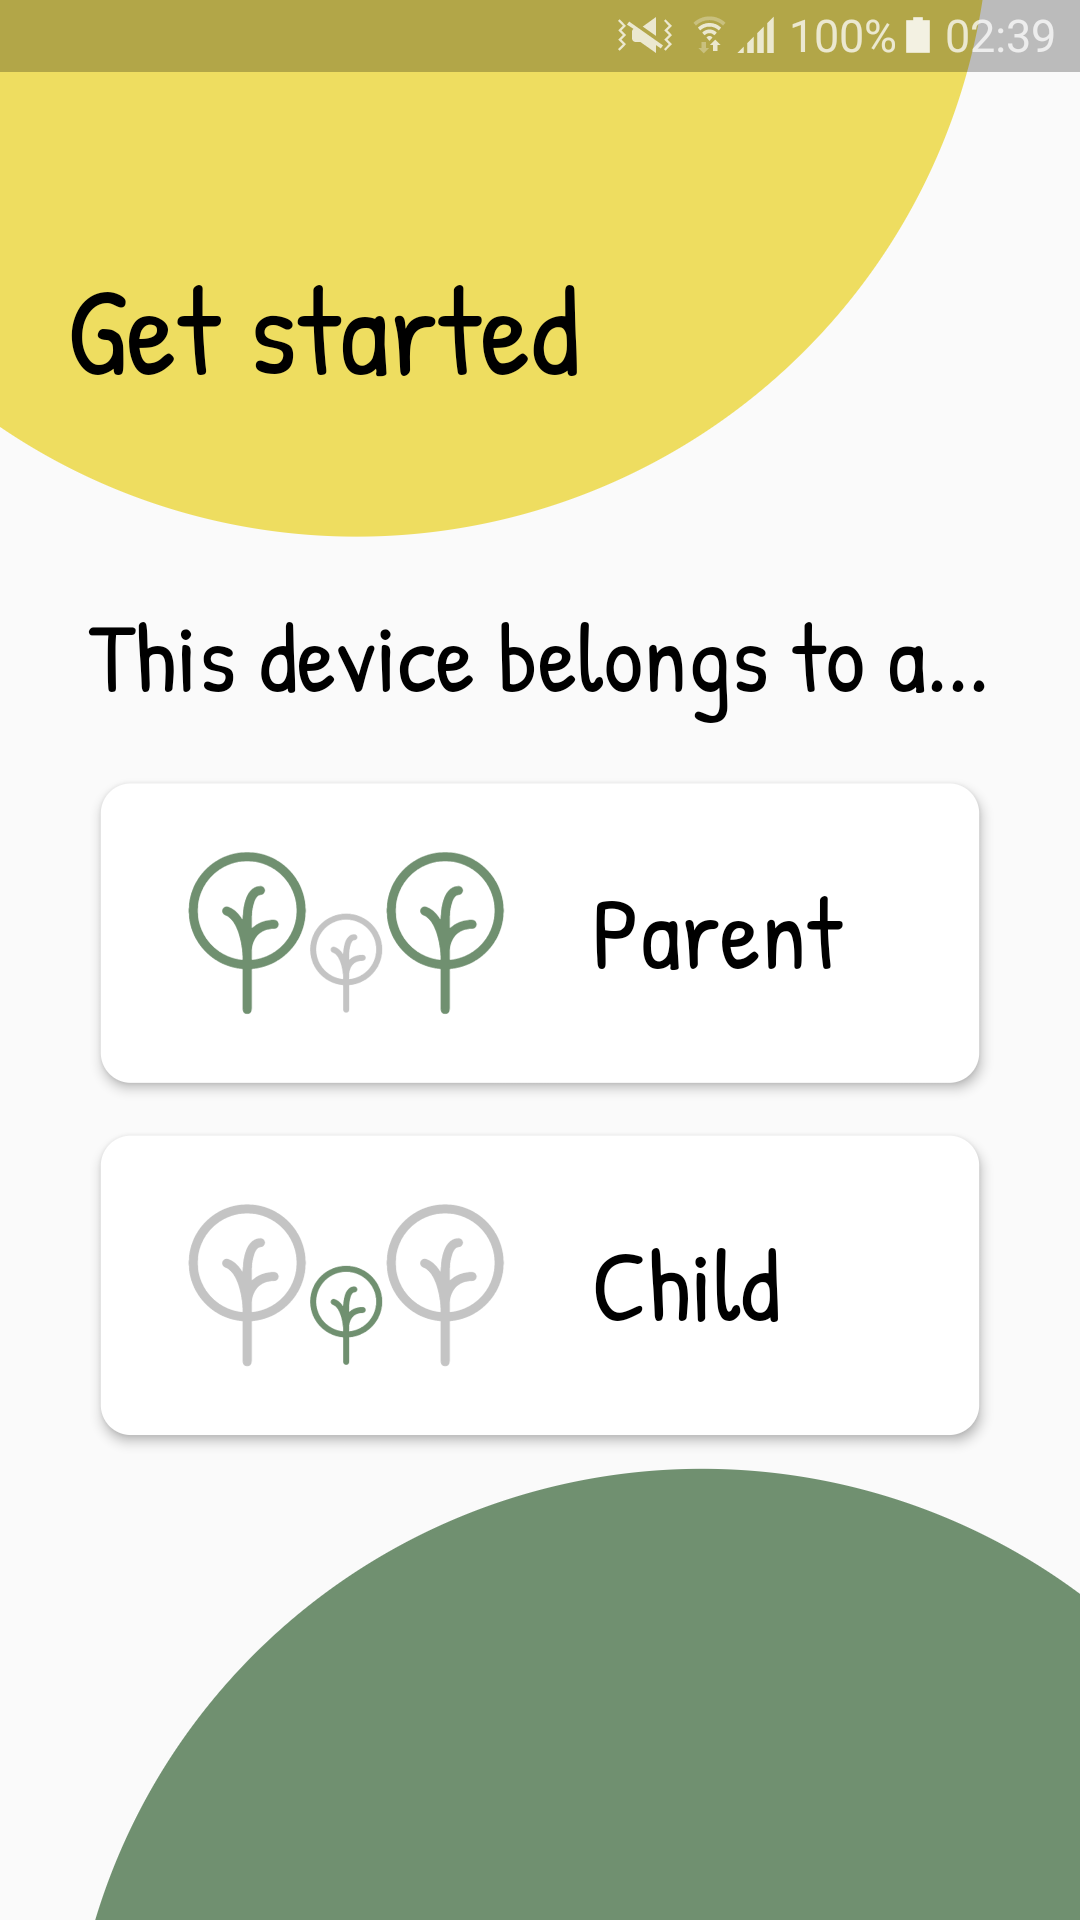
\includegraphics[width=.295\linewidth]{images/cross-device/SGS5/belonging.png}} 
&
\subcaptionbox{Login screen\label{fig:cross-device:sgs5:login}}{ 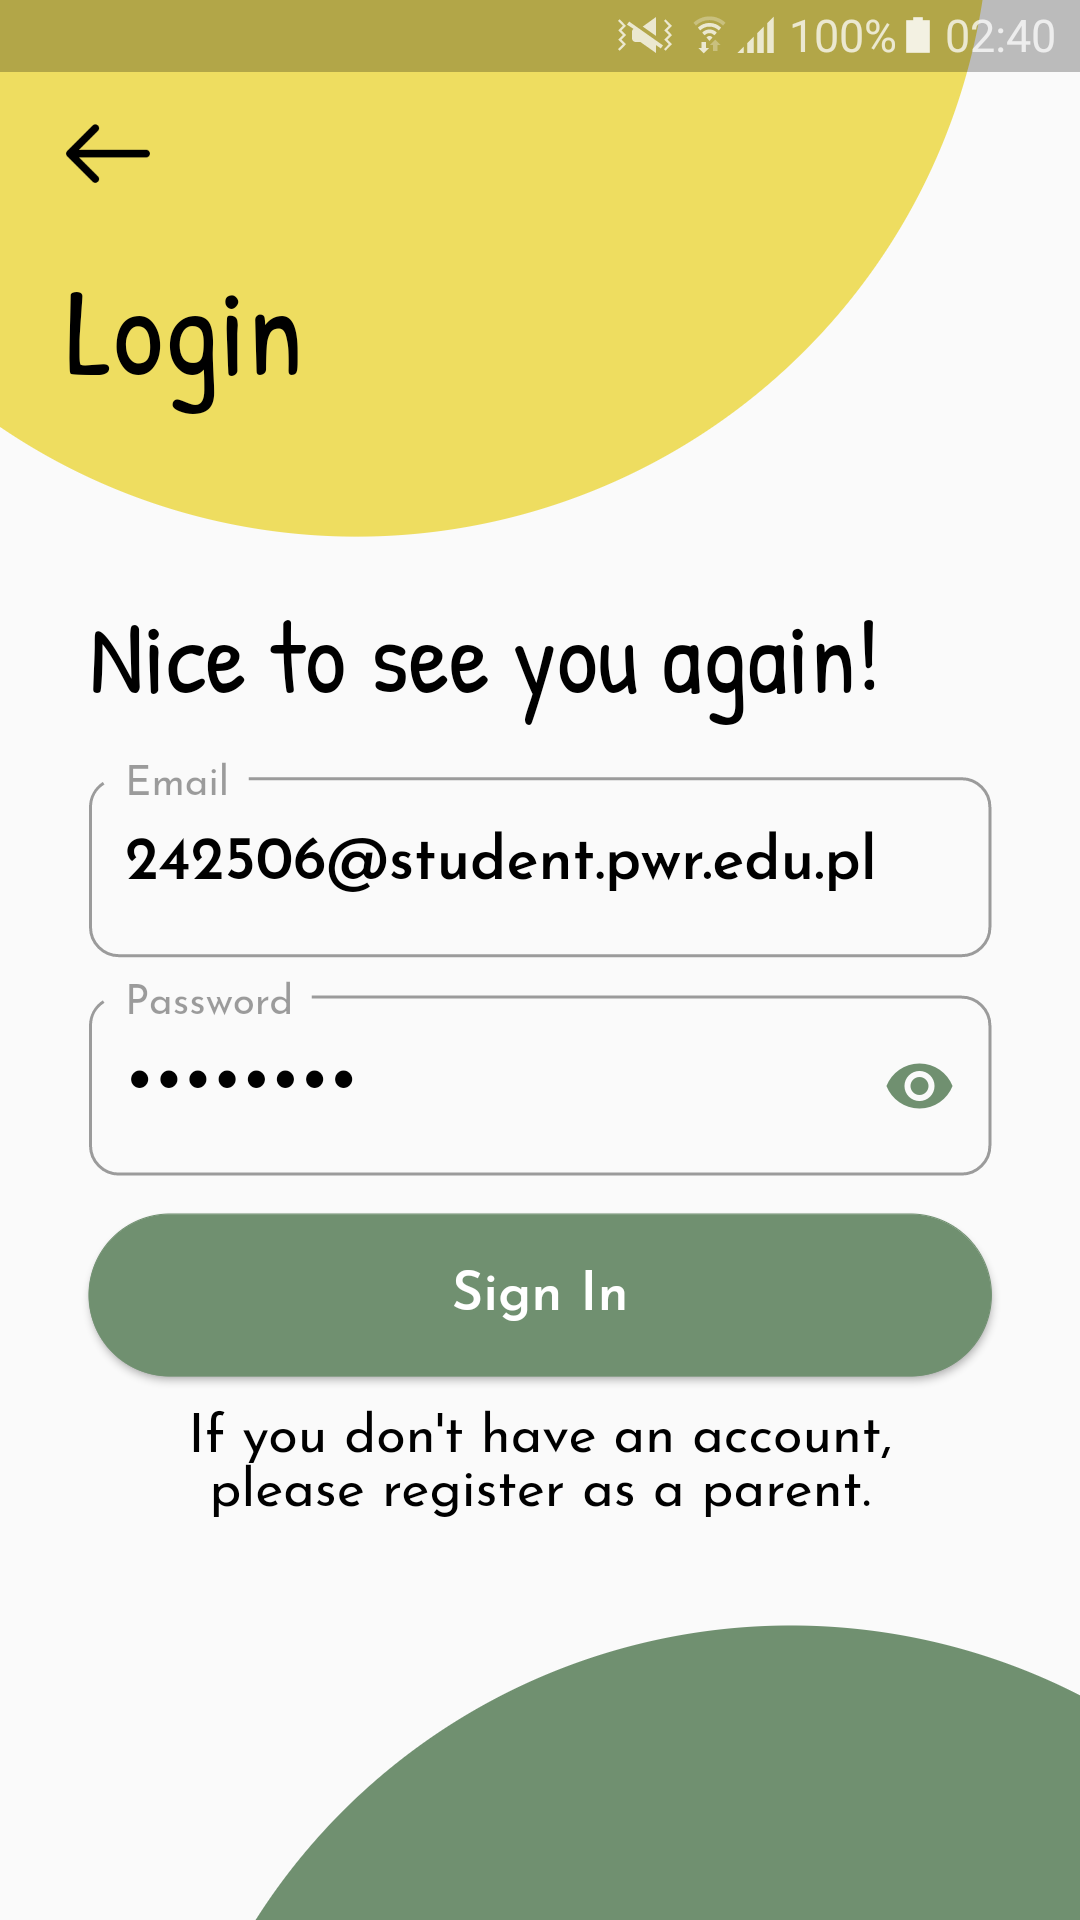
\includegraphics[width=.295\linewidth]{images/cross-device/SGS5/login.png}} 
&
\subcaptionbox{Children's profiles list screen\label{fig:cross-device:sgs5:profiles}}{ 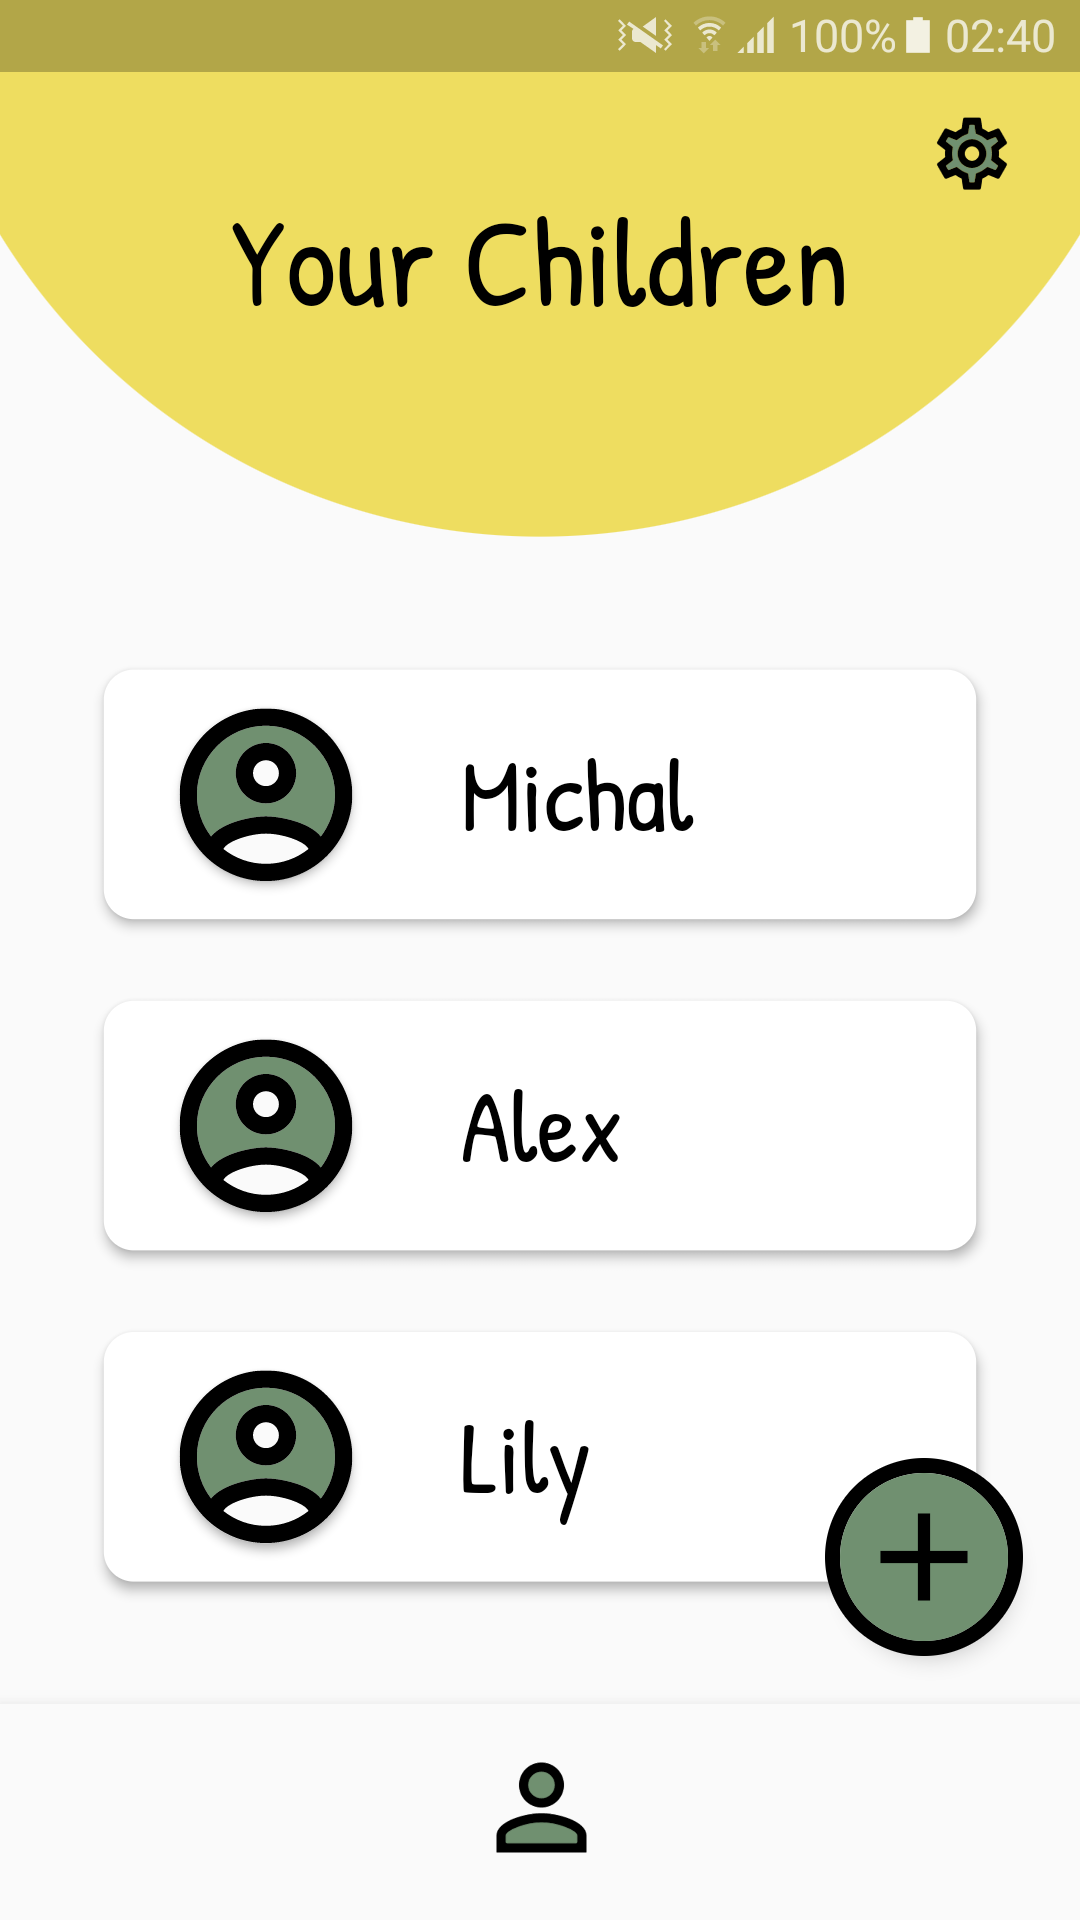
\includegraphics[width=.295\linewidth]{images/cross-device/SGS5/profiles.png}} 

\\\\\\\\
\subcaptionbox{Child's tasks screen\label{fig:cross-device:sgs6:tasks}}{ 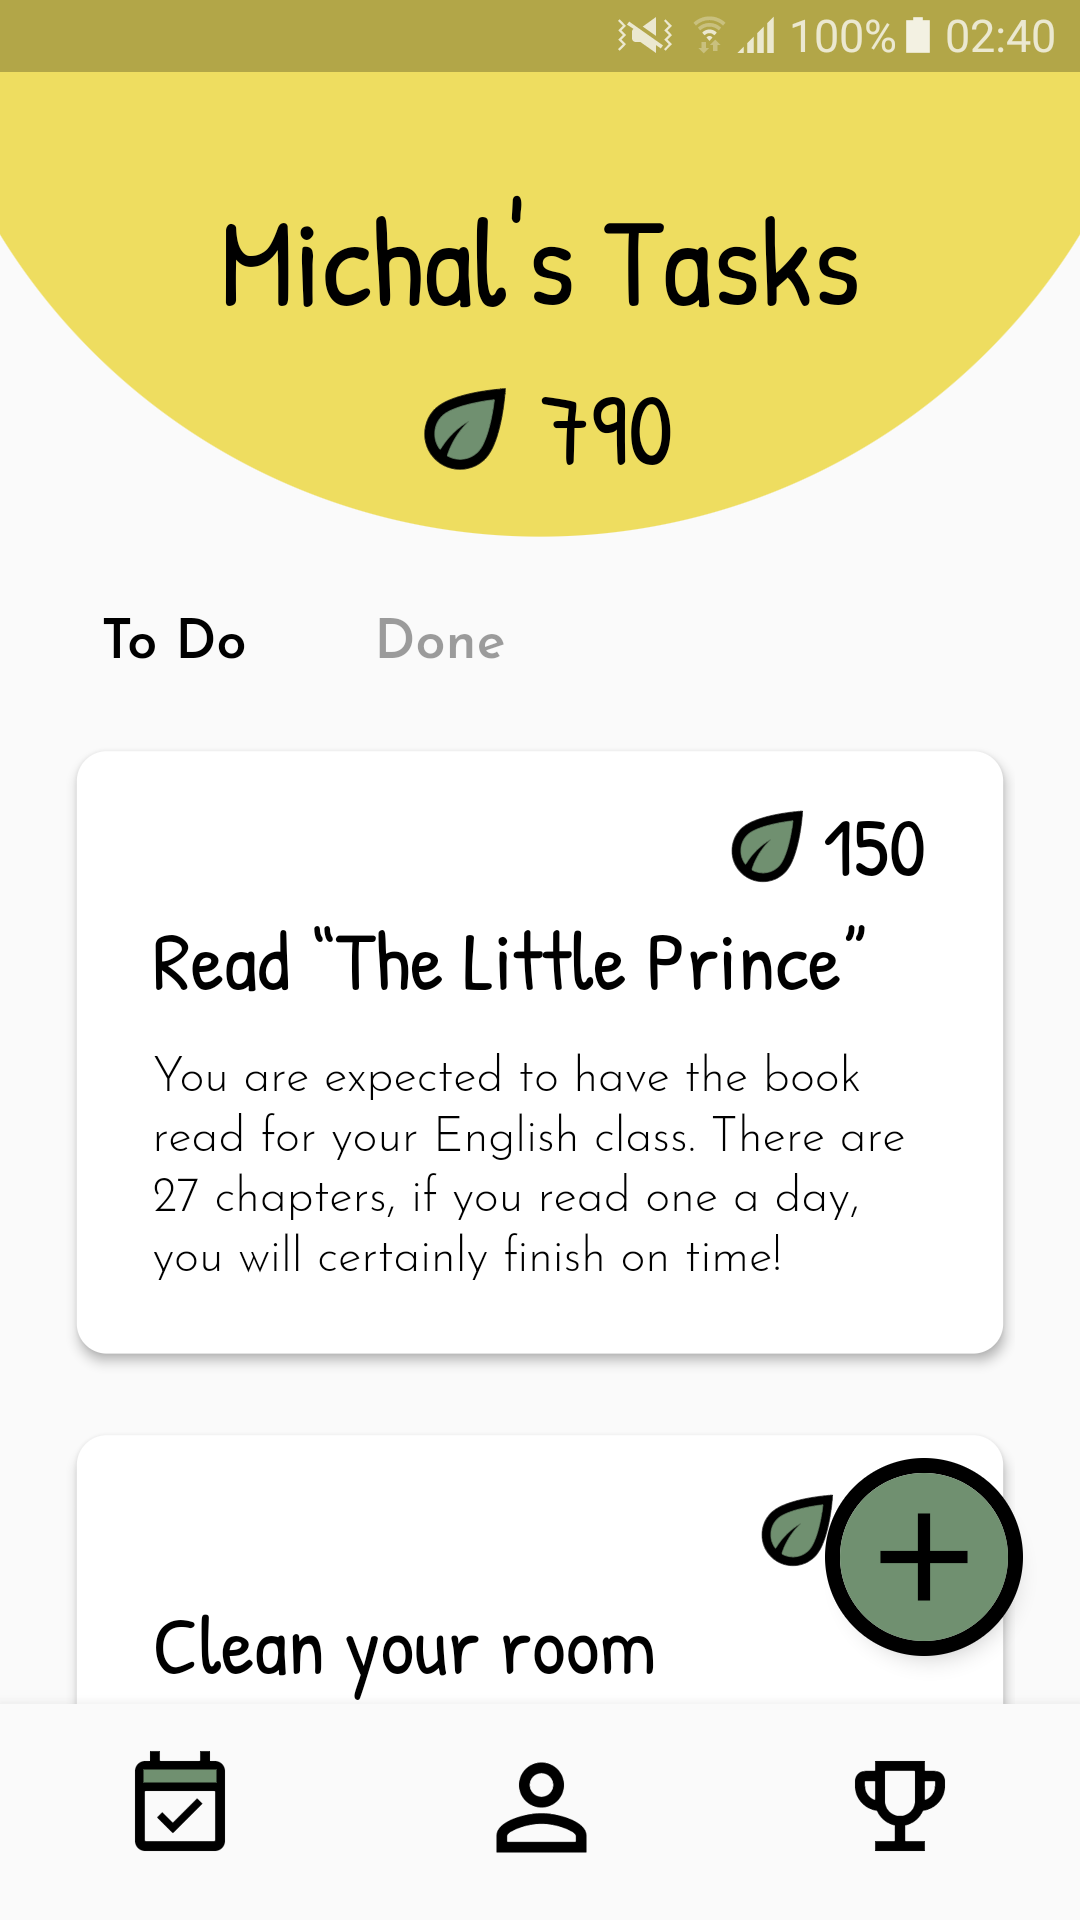
\includegraphics[width=.295\linewidth]{images/cross-device/SGS5/tasks.png}} 
&
\subcaptionbox{Task edit screen\label{fig:cross-device:sgs5:edit-task}}{ 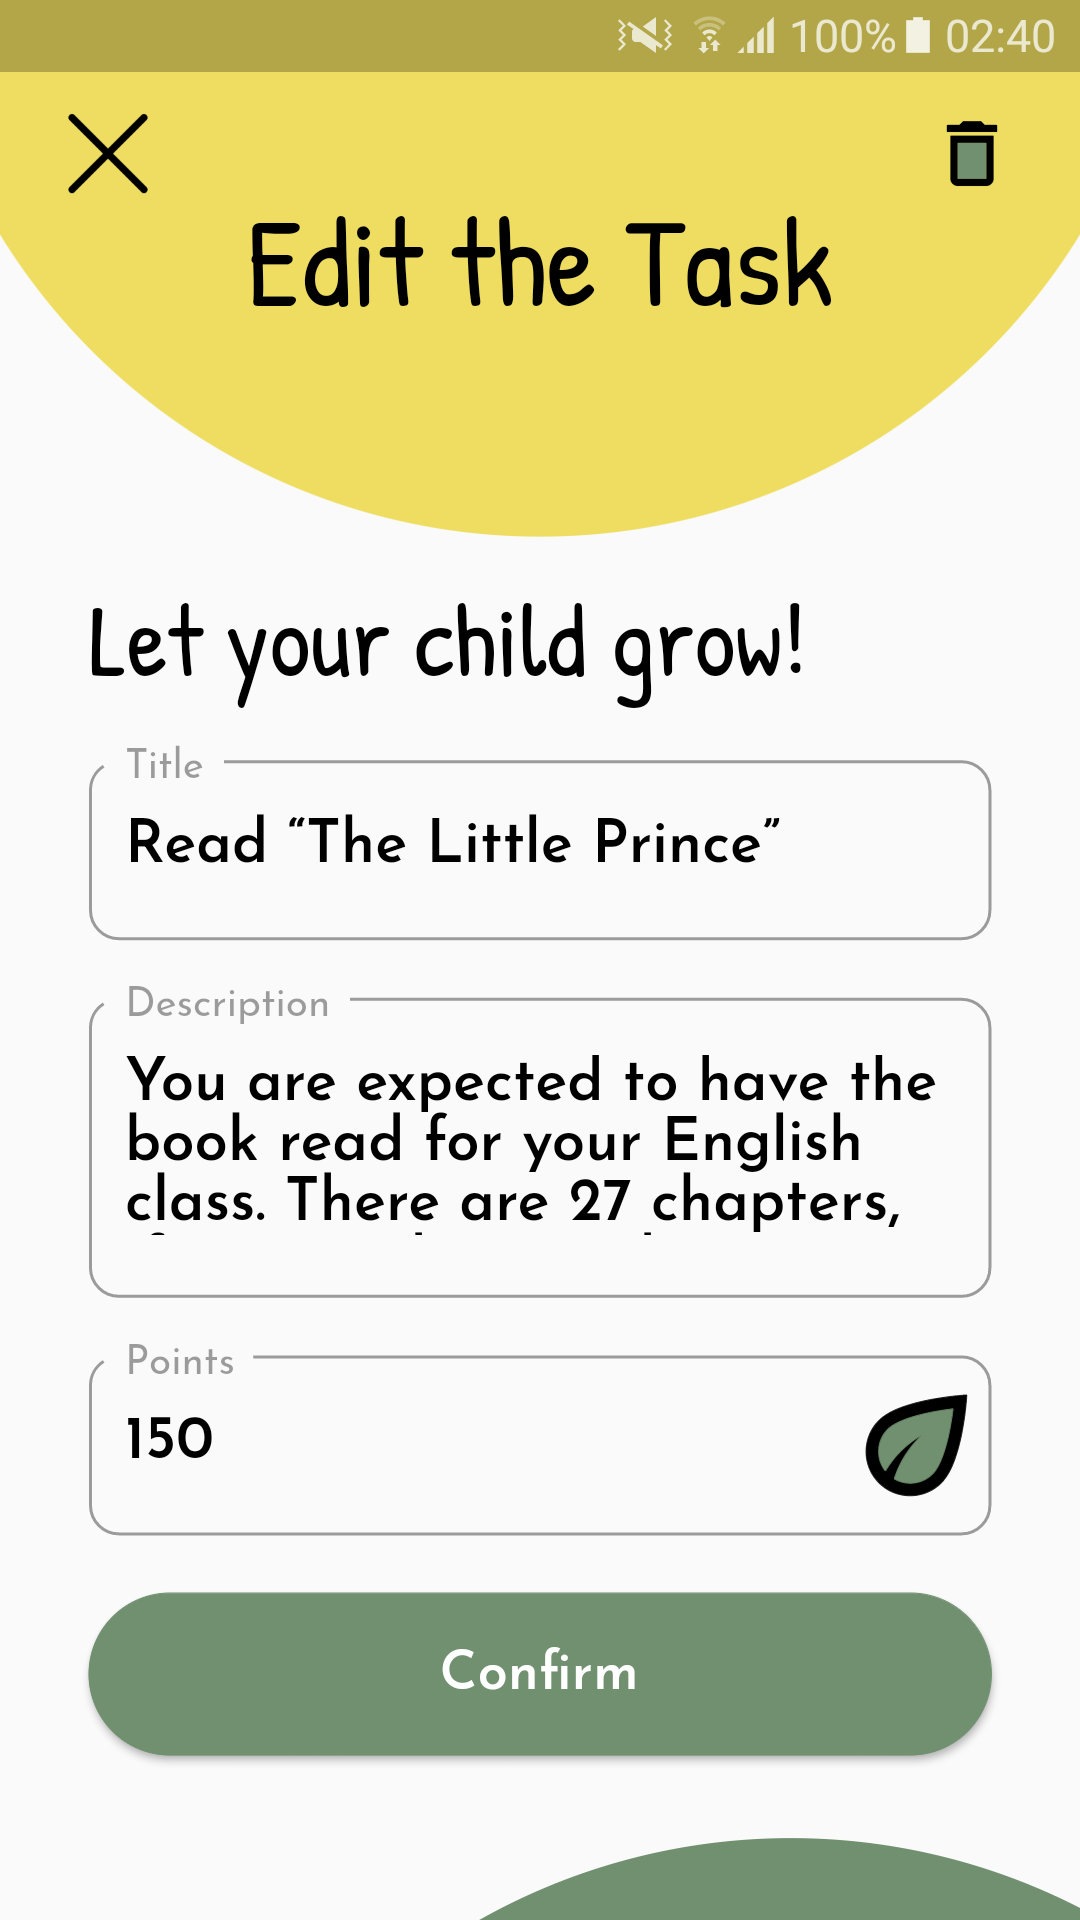
\includegraphics[width=.295\linewidth]{images/cross-device/SGS5/edit_task.png}} 
&
\subcaptionbox{Delete task confirmation\label{fig:cross-device:sgs5:delete-task}}{ 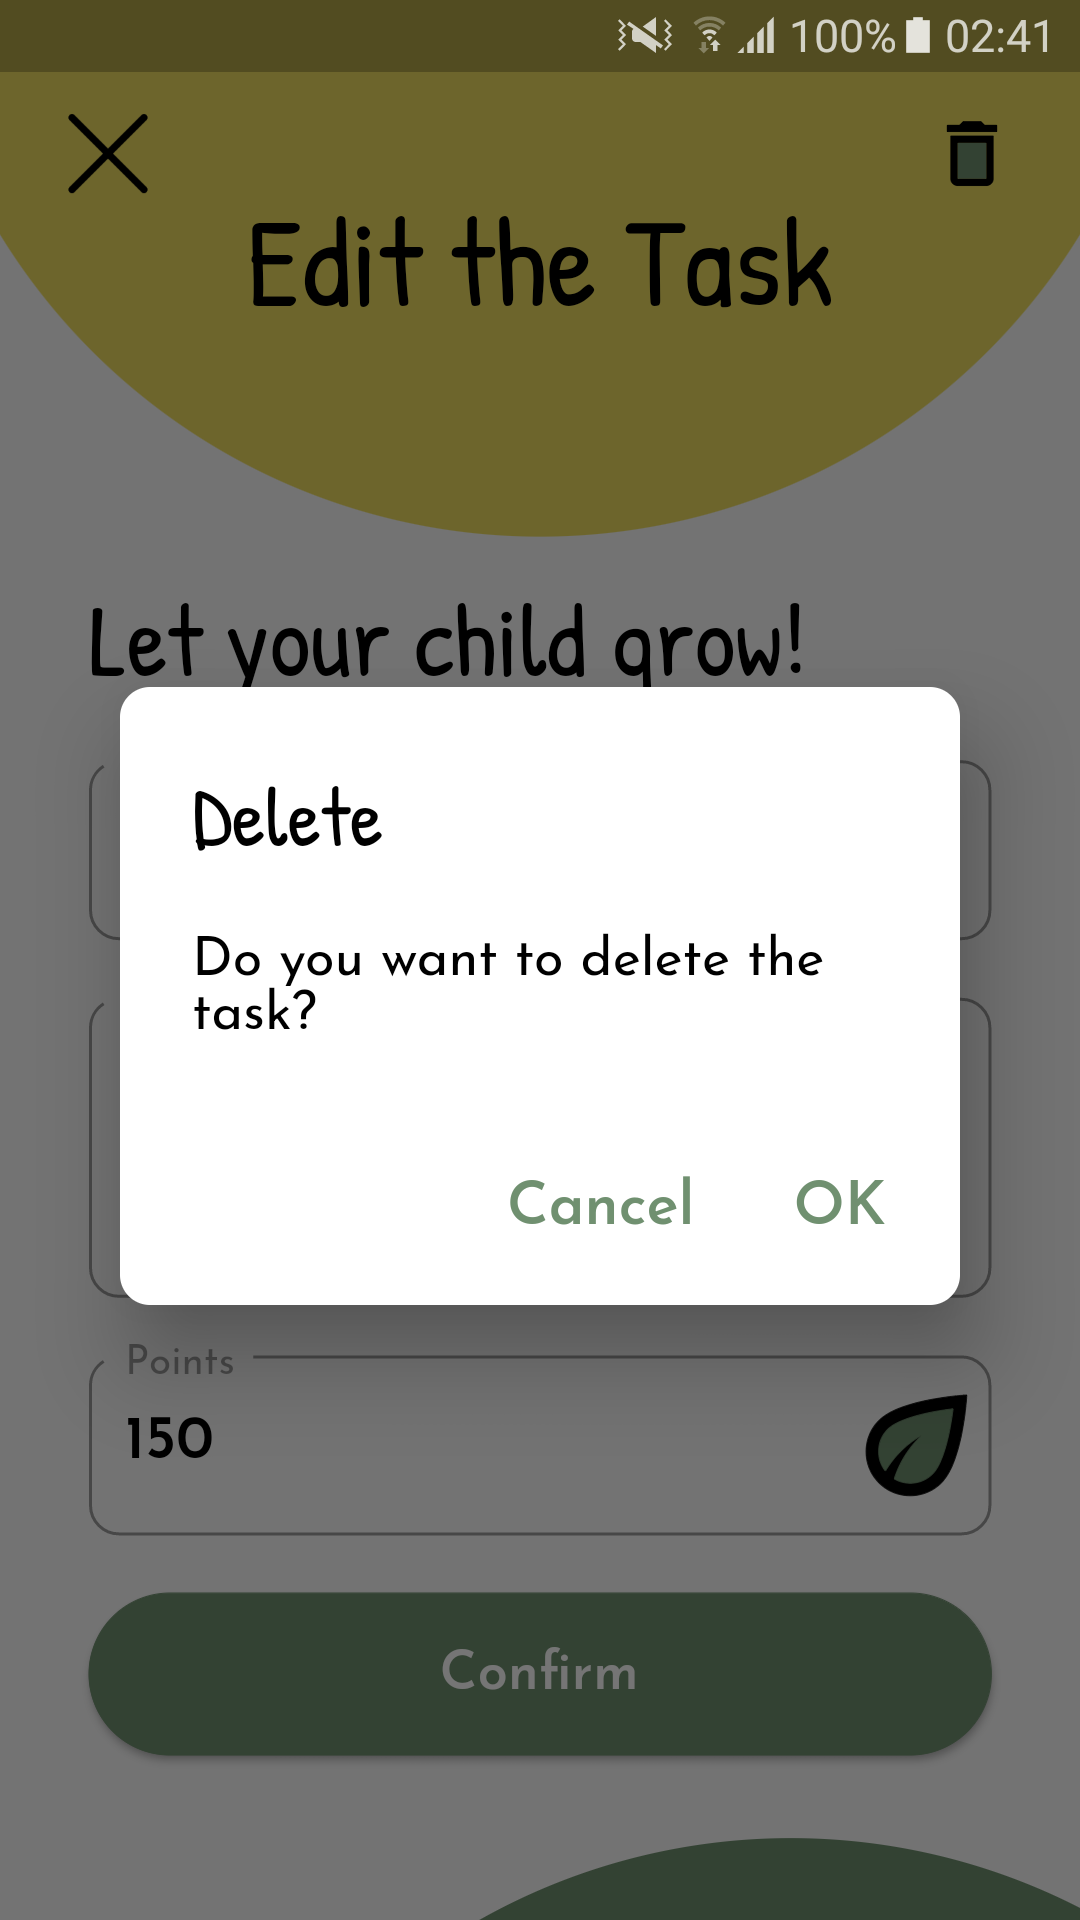
\includegraphics[width=.295\linewidth]{images/cross-device/SGS5/delete_task.png}} 
\end{tabular}
\caption{\textit{Raise App} selected screens displayed on Samsung Galaxy S5}
\label{fig:cross-device:sgs5}
\end{figure}